
The controller structure derived from this technique is similar to the pole placement one, but a significant conceptual difference exists. In fact, the linear quadratic regulator~(LQR) is obtained by optimizing the cost function~(\ref{eq:LQ_cost_function}) that includes both state and output, weighted by~$Q$ and~$R$ matrices respectively.
\begin{equation}
	J(x_0, u) = \int_{0}^{+\infty} \bigl{[} x'(\tau)Qx(\tau) + u'(t)Ru(t) \bigr{]} \; d\tau
	\label{eq:LQ_cost_function}
\end{equation}

The time horizon is infinite, so the solution~$\bar{P}$ of the \textit{algebraic Riccati equation}~(\ref{eq:LQ_ARE}) is constant and returns the time-invariant control law~(\ref{eq:LQ_control_law}).
\begin{subequations}
	\begin{equation}
		0 = A' \bar{P} + \bar{P} A + Q - \bar{P} B R^{-1} B' \bar{P}
		\label{eq:LQ_ARE}
	\end{equation}
	\begin{equation}
		u(t) = -K x(t)
		\label{eq:LQ_control_law}
	\end{equation}
\end{subequations}

The system response, such as settling time and transient shape, highly depends on mutual ratios between values in those matrices, that become design parameters. Many simulations in Simulink allowed us to find a possible trade-off among those parameters, just to perform an acceptable experiment in laboratory and, starting from that, improve performances by tuning.
As done in pole placement, the system~(both in case~\acrshort{1-dof} and~\acrshort{2-dof}) has been enlarged so that an integrator is able to nullify the steady-state error.

\paragraph{\acrshort{1-dof} system}

Similarly to the pole-placement control, the state is enlarged by adding an integrator on the error:
\begin{equation}
	\begin{bmatrix}
		\dot{x} \\
		\dot{v}
	\end{bmatrix}
	=
	\begin{bmatrix}
		A_{sys} & 0 \\
		-C_{back} & 0
	\end{bmatrix}
	\begin{bmatrix}
		x \\
		v
	\end{bmatrix}
	+
	\begin{bmatrix}
		B_{sys} \\
		0
	\end{bmatrix}
	V
	\qquad
	where \; C_{back} =
	\begin{bmatrix}
		0 & 0 & -1 & 0 & 0
	\end{bmatrix}
\end{equation}

For the design of this control technique, performing simulations is essential to find a good trade-off between~$Q$ and~$R$ values: their balance is fundamental to simultaneously have a rapid smooth transient and negligible steady-state error. A great coefficient on the integral part imposes a fast response and small steady-state error; quite high values on the position variables~($\theta_l$ and~$\theta_1$) accelerate in reaching the equilibrium, i.e.\ the reference. \\ Further considerations about speeds weight are needed: a very small coefficient on~$\dot \theta_l$ and~$\dot \theta_1$ would encourage high-frequency speed variation and then oscillations; on the other hand, augmenting those coefficients would speed-down the response, since a velocity variation~(necessary to move the mass) is discouraged. In conclusion, speeds parameters are probably the most difficult to be found. \\ Matrix~$R$ acts on the control variable usage: a too small coefficient causes rapid oscillations on voltage, a high value imposes a loose control action.
Here the matrices found by simulation:
\begin{equation}
	Q =
	\begin{bmatrix}
		50 & 0 & 0 & 0 & 0 \\
		0 & 0.1 & 0 & 0 & 0 \\
		0 & 0 & 50 & 0 & 0 \\
		0 & 0 & 0 & 0.1 & 0 \\
		0 & 0 & 0 & 0 & 3000 \\
	\end{bmatrix}
	\qquad
	R = 0.8
\end{equation}

The control law, hence, depends on both the state~$x(t)$ and the integral variable~$v(t)$. Since not all measurements are available~(speeds are very noisy), a state reconstructor is necessary: the Kalman Filter introduced in chapter~4 works thanks to~$\theta_l$ and~$\theta_1$ signals, that makes this LQR an LQG control. As shown in figure~\ref{fig:1dof_LQ_classicKF}, from the simulation a settling time of~0.8~s~(comparable to the previous controllers, but greater than the one of Kalman Filter, as desired) is expected. Actually, laboratory experiment is a bit oscillating in the transient; indeed, this control technique does not explicitly cancel the system dynamics, difficult to be attenuated by tuning matrices. At steady-state condition, the integral action could detect a small static error that would cause some sudden motions, so a switch disables the input signal of the integrator in proximity of the reference.

\begin{figure*}
	\centering
	\begin{subfigure}{0.45\columnwidth}
		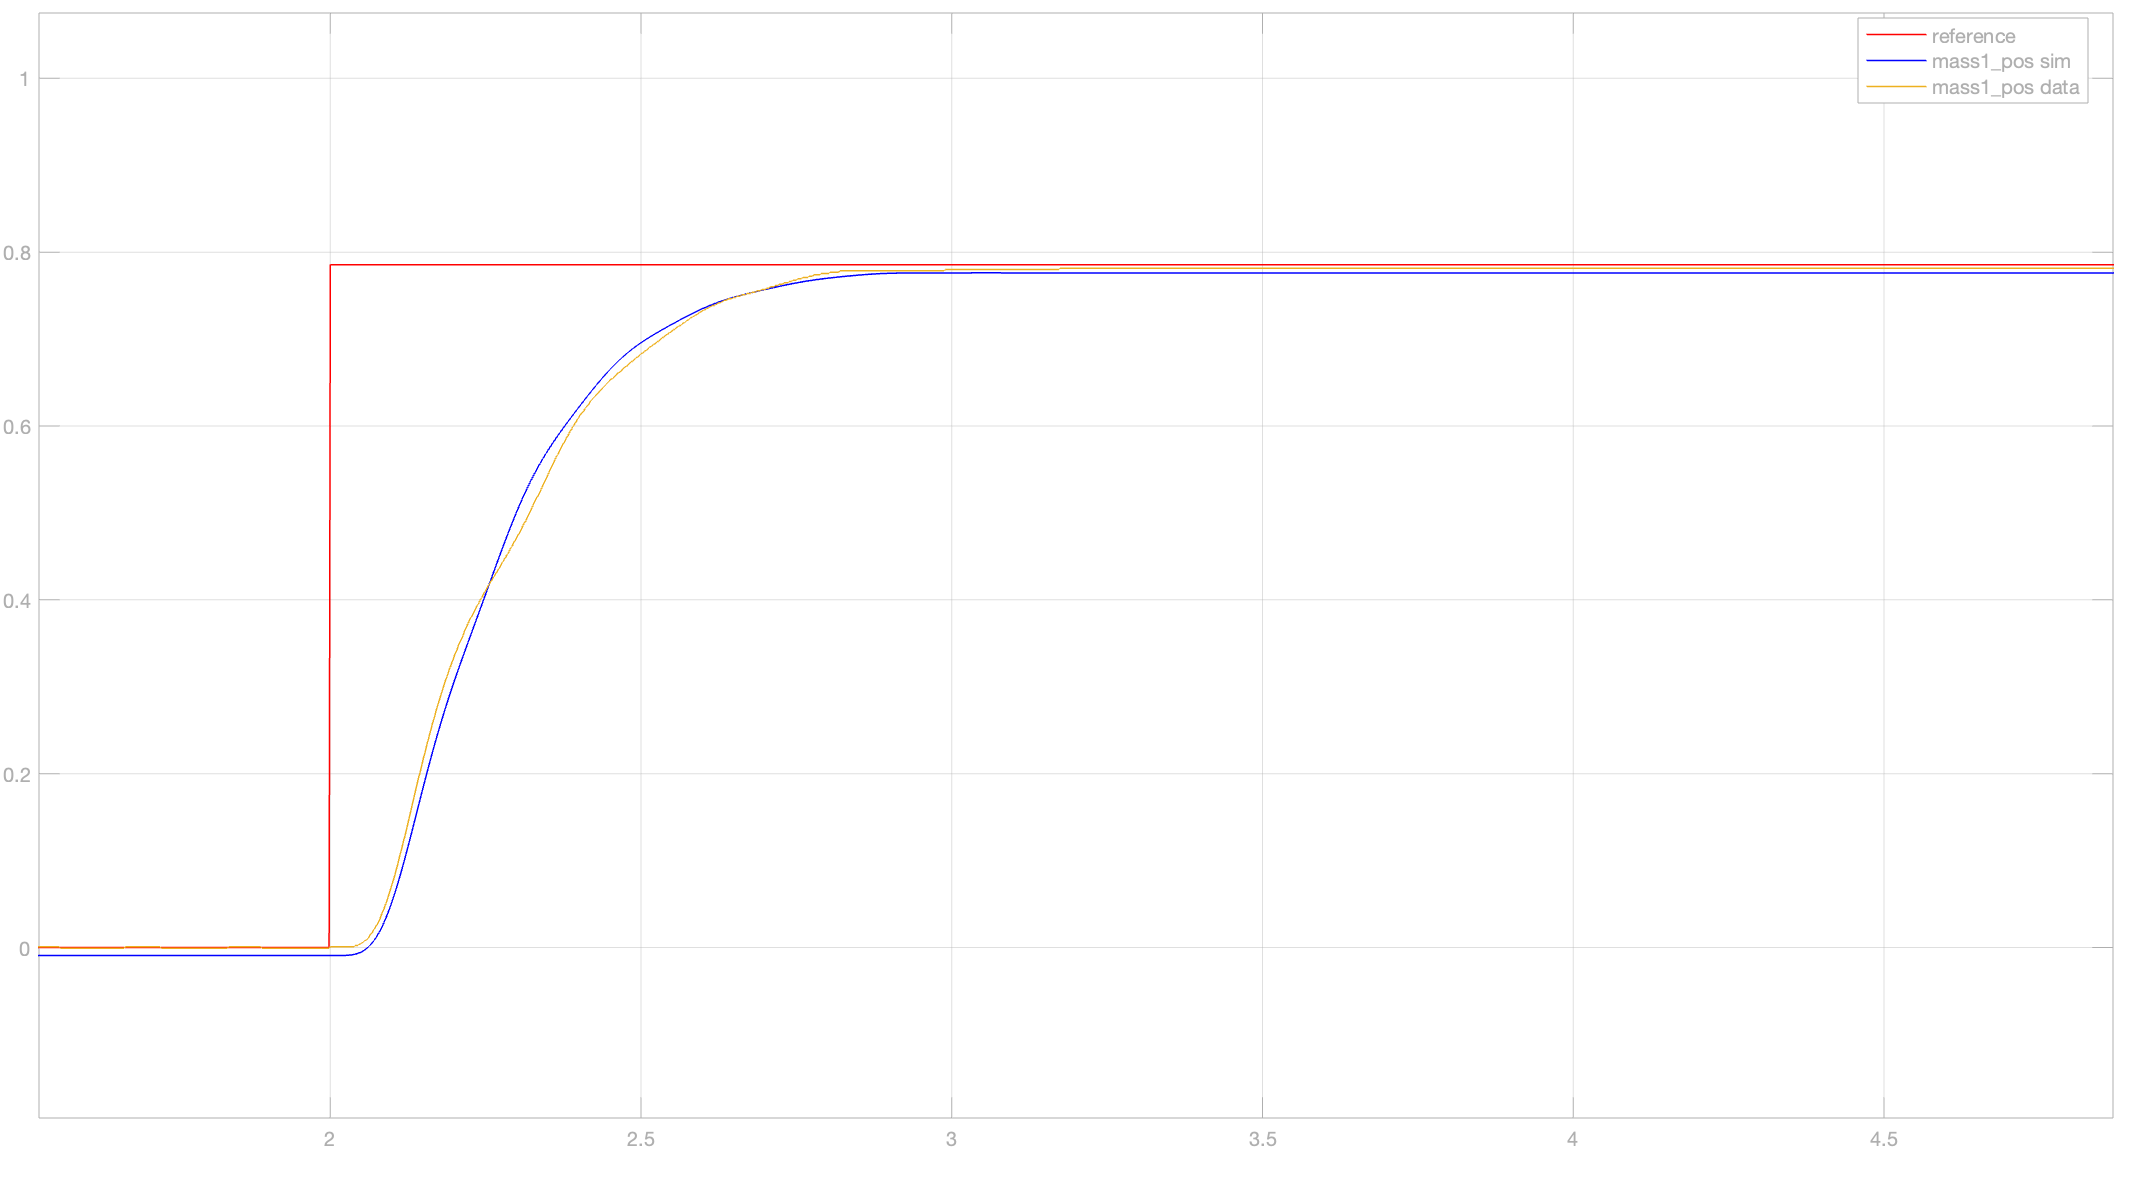
\includegraphics[width=\textwidth]{1dof_LQ_classicKF}
		\subcaption{LQG with all measurements}
		\label{fig:1dof_LQ_classicKF}
	\end{subfigure}
	\begin{subfigure}{0.45\columnwidth}
		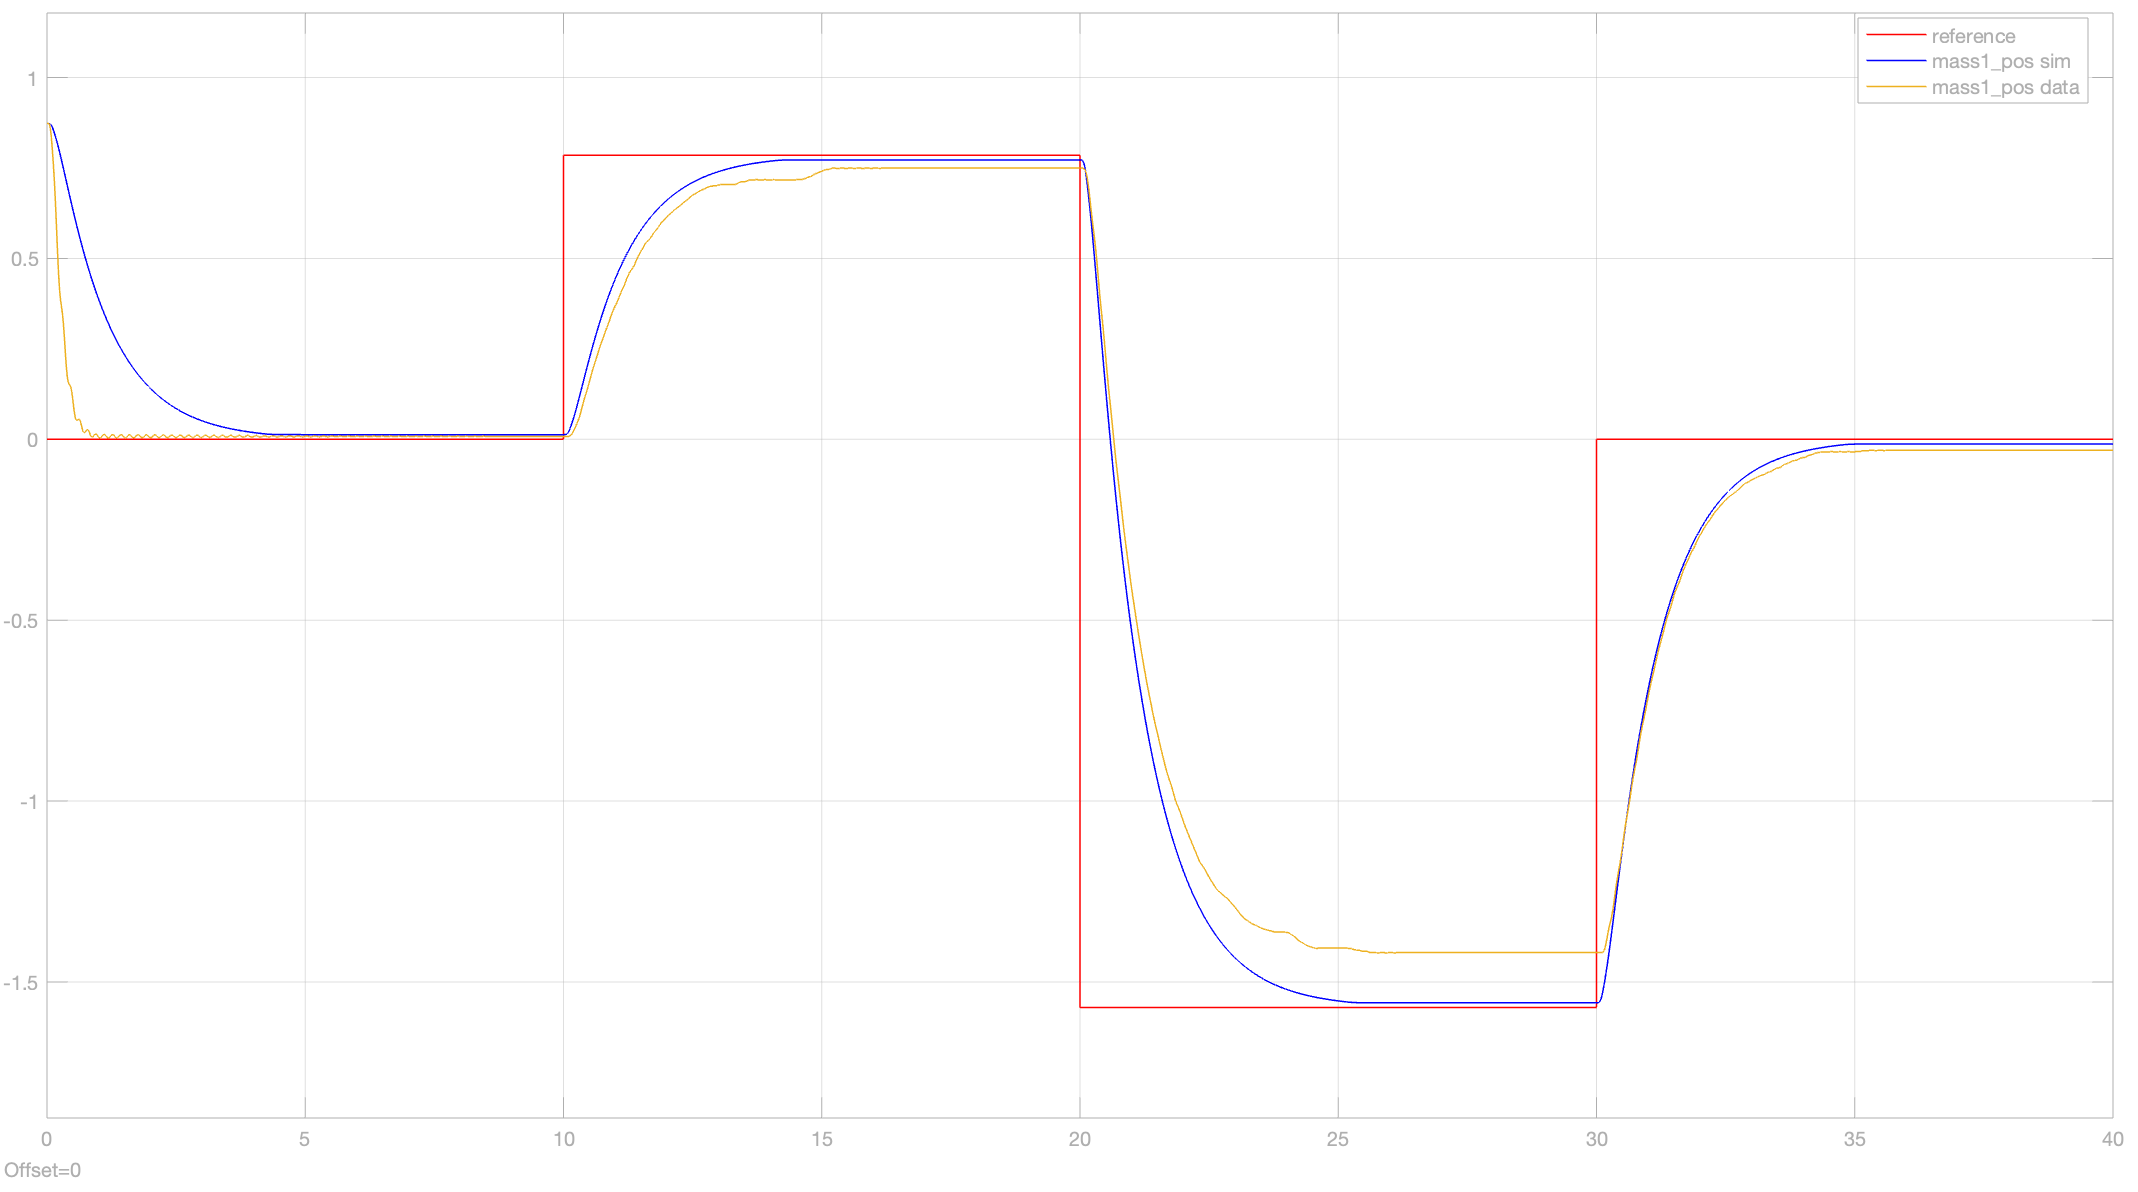
\includegraphics[width=\textwidth]{1dof_LQ_minKF_pot}
		\subcaption{LQG with potentiometer sensor only}
		\label{fig:1dof_LQ_minKF_pot}
	\end{subfigure}
	\newline
	\begin{subfigure}{\columnwidth}
		\centering
		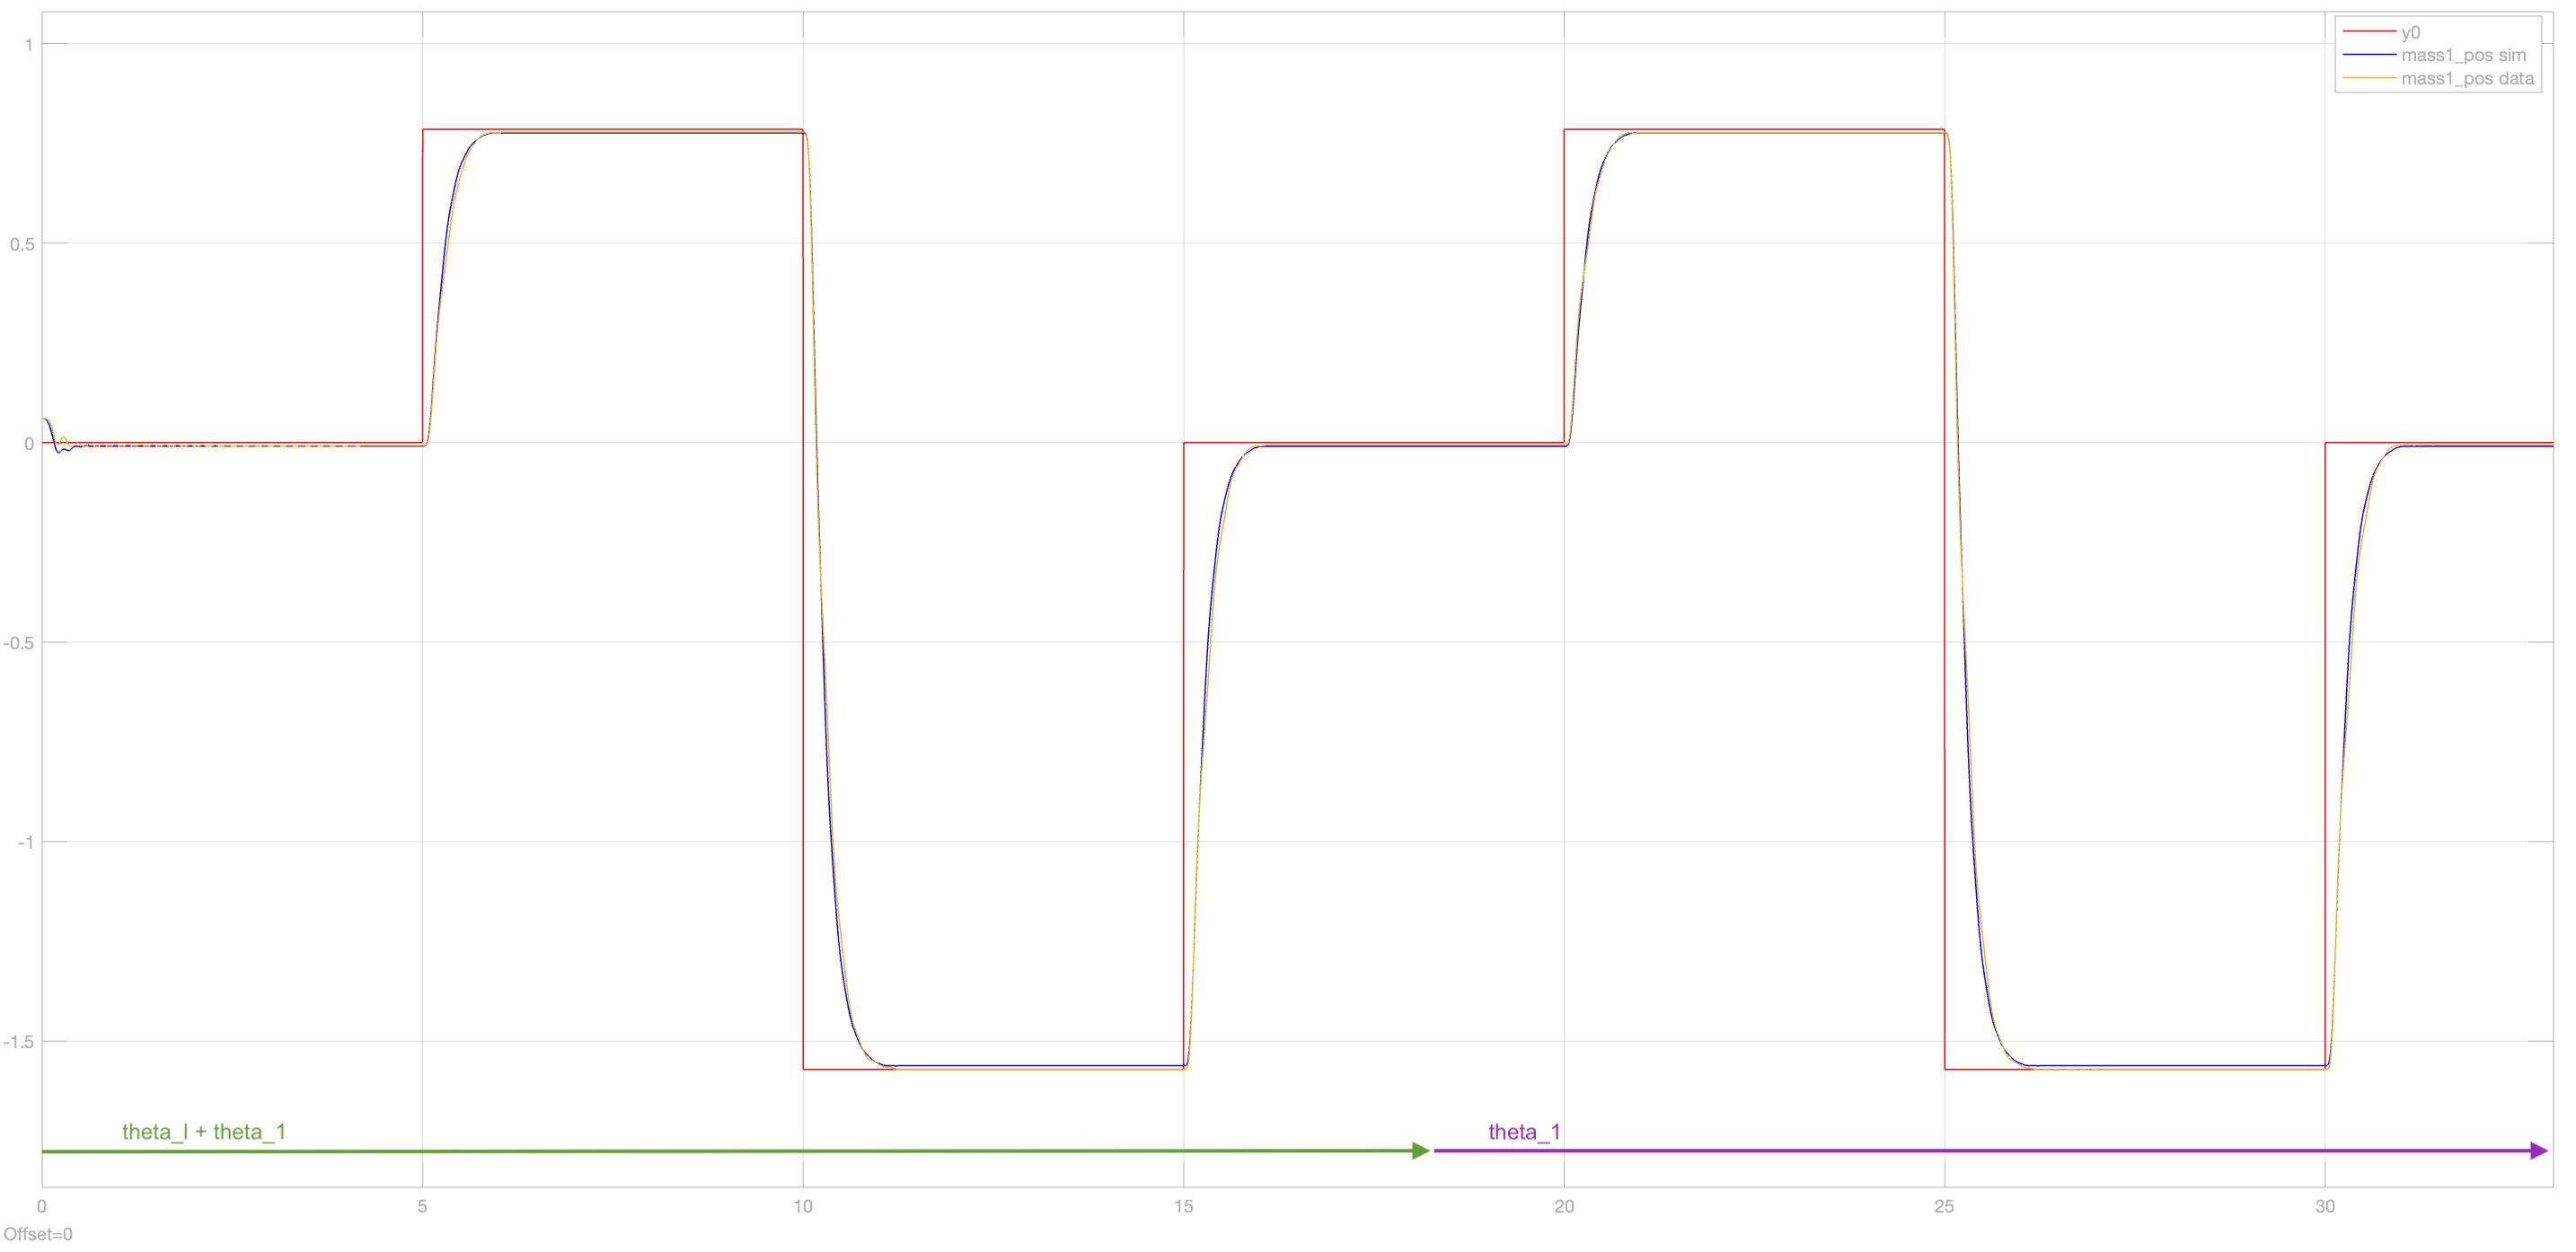
\includegraphics[width=0.9\textwidth]{1dof_LQ_KF_switch}
		\subcaption{LQG with switch among different KF}
		\label{fig:1dof_LQ_KF_switch}
	\end{subfigure}
	\caption{LQG with different sensors available, \acrshort{1-dof} case}
\end{figure*}

\subparagraph{Sensors not available: minimum Kalman Filters}

% verificare concordanza con spiegazione minKF in capitolo 4
Now we consider the case of missing signals, possibly due to sensor faults or installation impossibility. In this case, the Kalman Filters structure changes, as explained in chapter~4. In case the signal of the last mass, here~$\theta_1$, is not available, the reference error is computed on the estimation of that signal~($\hat\theta_1$), figure~\ref{fig:KF_state_feedback}. \\

\begin{figure*}
	\centering
	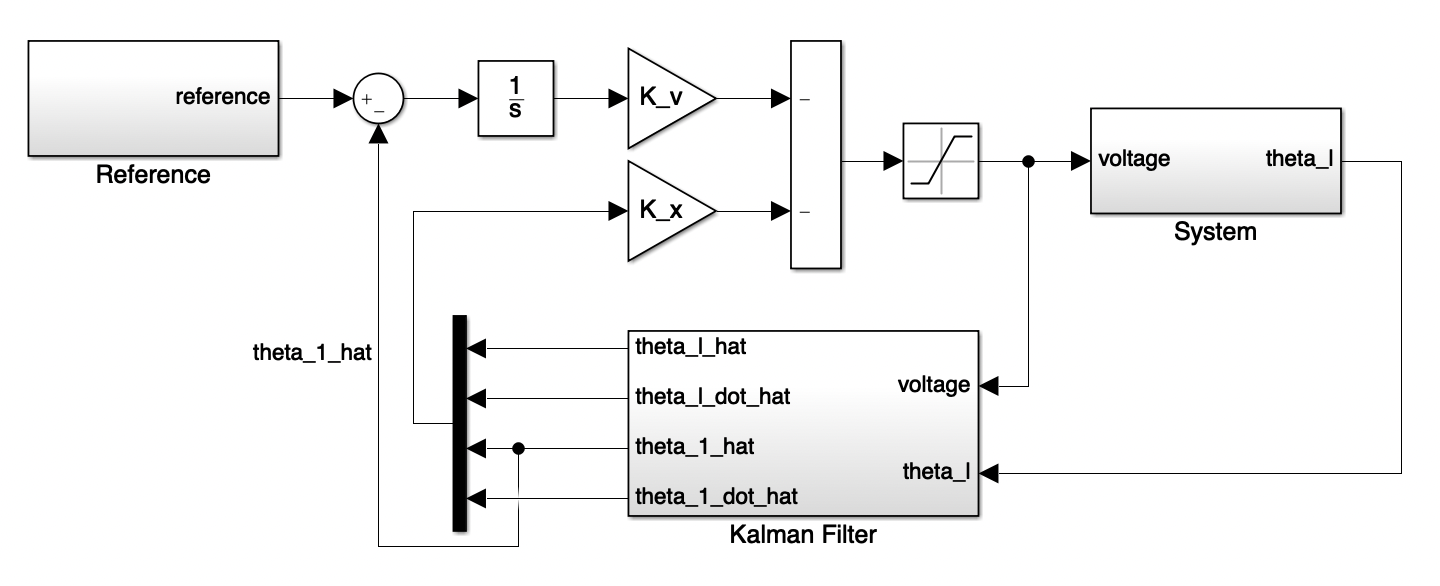
\includegraphics[width=0.8\textwidth]{KF_state_feedback}
	\caption{State measurement not available: estimated state feedback, \acrshort{1-dof} case}
	\label{fig:KF_state_feedback}
\end{figure*}

In order to speed up the laboratory experience, a long experiment that switches among the different combinations of available sensors has been performed; this simulates a real-time fault detection and, accordingly, commutation to a congruous configuration of the reconstructor.

In the~\acrshort{1-dof} case, actually, there are three different situations: all sensors available (i.e.\~potentiometer and first mass encoder), encoder only~($\theta_l$), potentiometer only~($\theta_1$). Unfortunately, this last Kalman Filter is very slow because of the potentiometer noise, hence an \textit{ad hoc} slower controller must be designed~(settling time~4~s, comparable with the Kalman time response):
\begin{equation}
	Q =
	\begin{bmatrix}
		50 & 0 & 0 & 0 & 0 \\
		0 & 1 & 0 & 0 & 0 \\
		0 & 0 & 50 & 0 & 0 \\
		0 & 0 & 0 & 1 & 0 \\
		0 & 0 & 0 & 0 & 100
	\end{bmatrix}
	\qquad
	R = 0.8
\end{equation}

A switch between the faster and the last one controllers could create some issues: a small error in the state estimation would cause a jump in the control action~(that is determined by a different gain~
$
\begin{bmatrix}
	K_x & K_v
\end{bmatrix}
$), generating an instability. Therefore, the only potentiometer Kalman reconstructor has been tested apart from the others (figure~\ref{fig:1dof_LQ_minKF_pot}). The superimposition of Kalman and LQR transients causes some oscillations in reaching the reference. Moreover, because of the error generation based on state reconstruction, the reference could not be reached if the step is significant; this is mainly due to the potentiometer loose performances and, probably, non-linear readings in some regions. It is notable that this is the only case where simulation and experiment significantly differ.

The long switching experiment, in figure~\ref{fig:1dof_LQ_KF_switch}, shows the other two possible situations: in the first 18~s all position sensors are available, then only the encoder is available.

\paragraph{\acrshort{2-dof} system}

In this case, the error is computed on the second mass position, then the enlarged system is formed by
\begin{equation}
	C_{back} =
	\begin{bmatrix}
		0 & 0 & 0 & 0 & 0 & -1 & 0
	\end{bmatrix}
\end{equation}

The additional parameters make the tuning more complicated. Here, a higher weight on the second mass position has been assigned, so that the transient on the reference (imposed to~$\theta_2$) is limited without affecting the motor and first mass dynamics: a very fast transient of the other components of the system could affect the desired behavior of the second mass (expecially time response and oscillations) and, in any case, would hide the integral contribution in the cost function, making the step response slower.
\begin{equation}
	Q = diag
	\bigl{(}
	\begin{bmatrix}
		10 & 0.8 & 10 & 0.8 & 80 & 0.8 & 4500
	\end{bmatrix}
	\bigr{)}
%	\begin{bmatrix}
%		10 & 0 & 0 & 0 & 0 & 0 & 0 \\
%		0 & 0.8 & 0 & 0 & 0 & 0 & 0 \\
%		0 & 0 & 10 & 0 & 0 & 0 & 0 \\
%		0 & 0 & 0 & 0.8 & 0 & 0 & 0 \\
%		0 & 0 & 0 & 0 & 80 & 0 & 0 \\
%		0 & 0 & 0 & 0 & 0 & 0.8 & 0 \\
%		0 & 0 & 0 & 0 & 0 & 0 & 4500
%	\end{bmatrix}
	\qquad
	R = 2.5
\end{equation}

In figure~\ref{fig:2dof_LQ_classicKF}, a comparison between simulation and experiment is visible. An improvement with respect to the~\acrshort{1-dof} case exists: no oscillations are present in the transient.

\subparagraph{Sensors not available: minimum Kalman Filters}

In this case, separate experiments are shown (figure~\ref{fig:2dof_LQ_minKF}) focusing on single step, so that the transients are more visible. It can be seen that all of them are very similar, meaning that the system is observable by using any of the proposed sensor combinations. \\
An issue appears by using Kalman Filter with potentiometer only: after a few seconds, an instability occurs and the experiment fails. There is a numerical reason for this, in fact from the mathematical viewpoint the \acrshort{2-dof}~system should be observable also from the potentiometer (checked by \textit{obsv}~Matlab function), but in practice it is not: performing the \textit{SVD} decomposition (result in~\ref{eq:2dof_minKF_pot_svd}), it is clear that at least two eigenvalues are negligible with respect to the dominant one.
\begin{equation}
	S = diag
	\bigl{(}
	\begin{bmatrix}
		4037,2 & 876.7 & 34.7 & 5.5 & 1 & 0.6
	\end{bmatrix}
	\bigr{)}
	\label{eq:2dof_minKF_pot_svd}
\end{equation}
This means that the only potentiometer is not sufficient for the state reconstruction and, so, for the control of the \acrshort{2-dof}~system.

\begin{figure*}
	\centering
	\begin{subfigure}{0.45\columnwidth}
		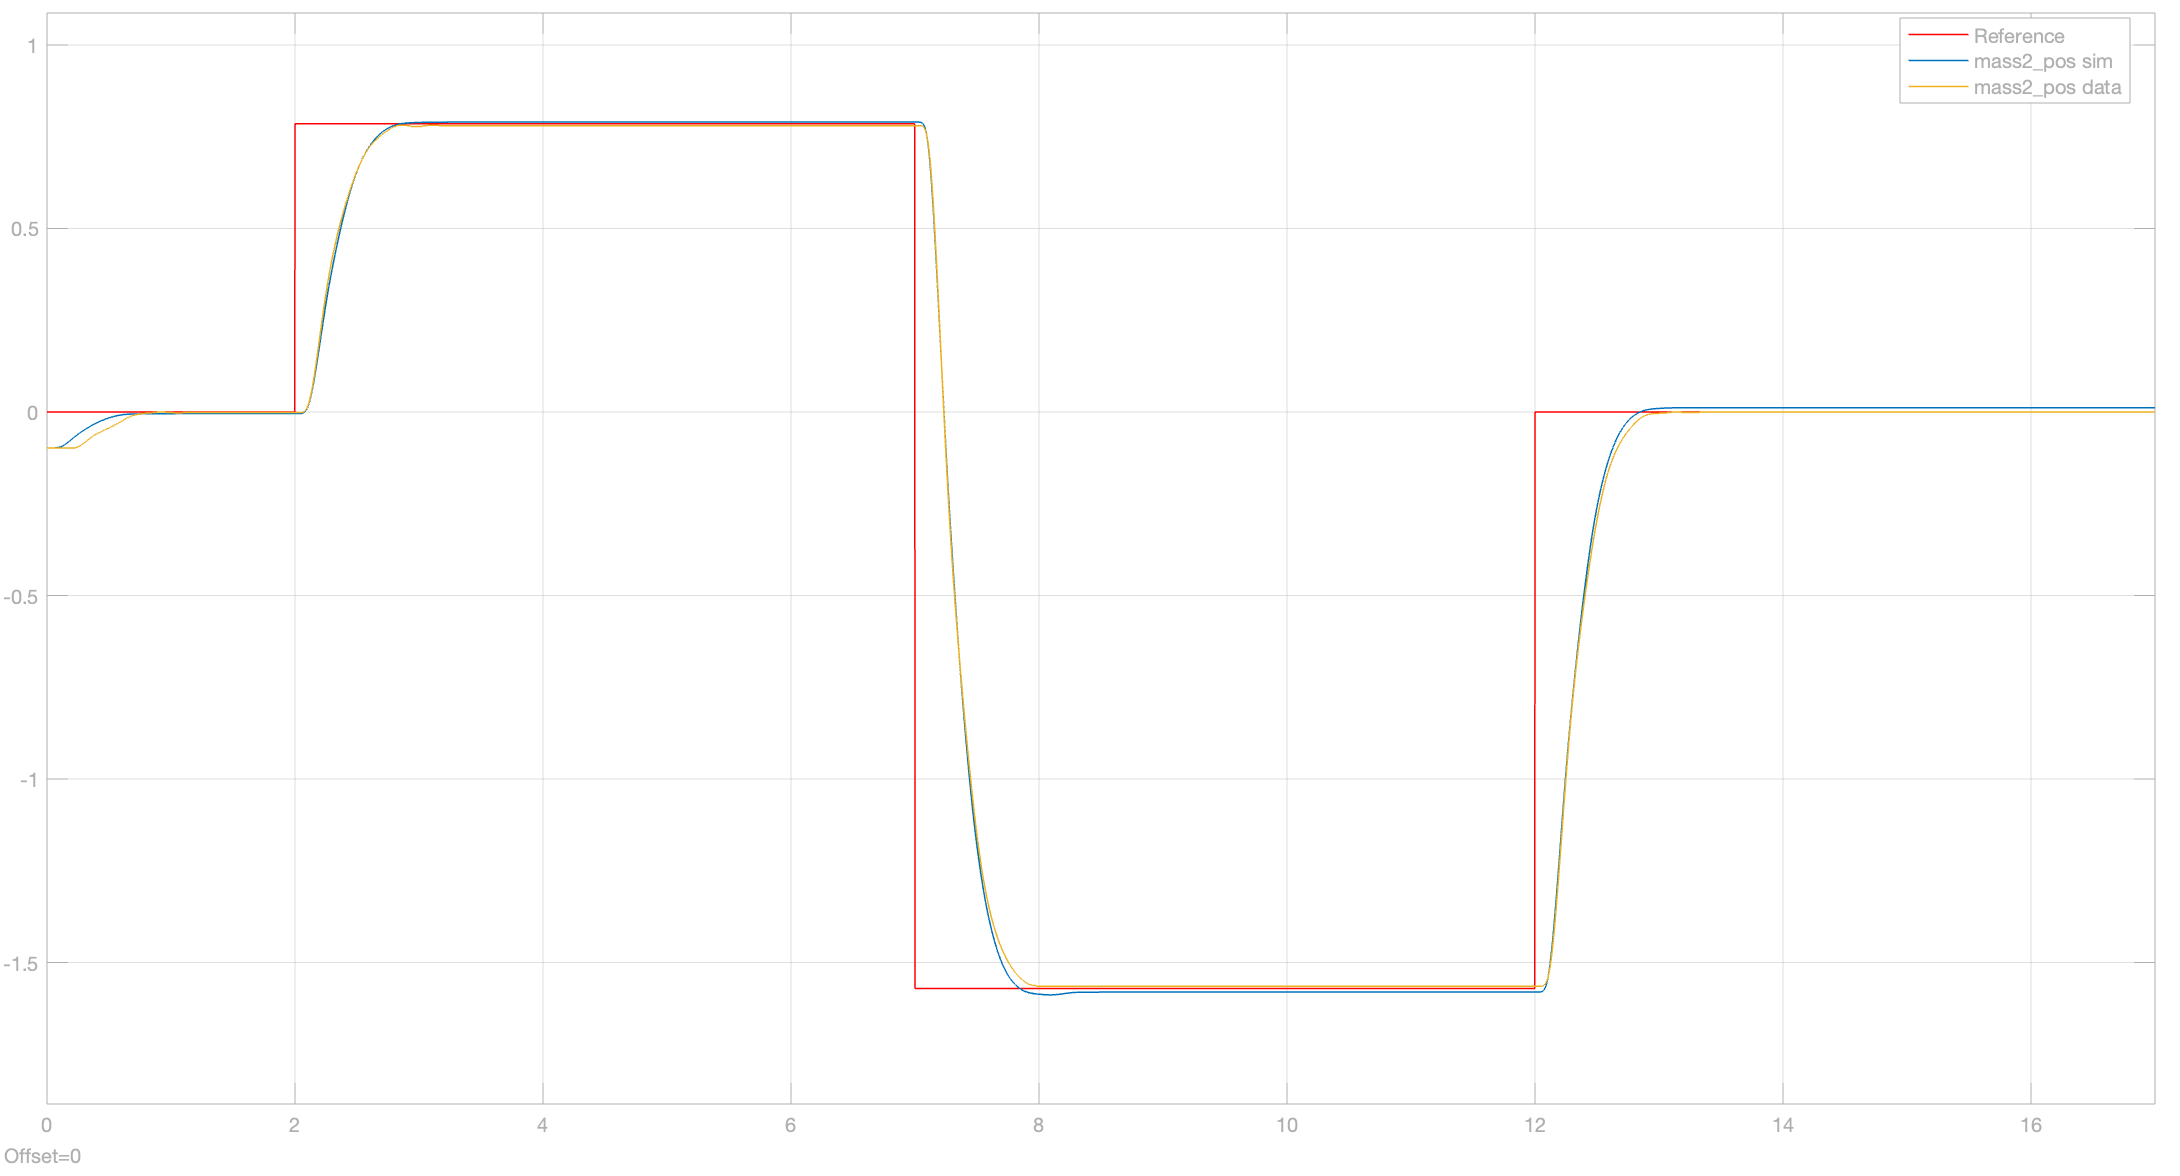
\includegraphics[width=\textwidth]{2dof_LQ_classicKF}
		\subcaption{LQG with all measurements}
		\label{fig:2dof_LQ_classicKF}
	\end{subfigure}
	\begin{subfigure}{0.45\columnwidth}
		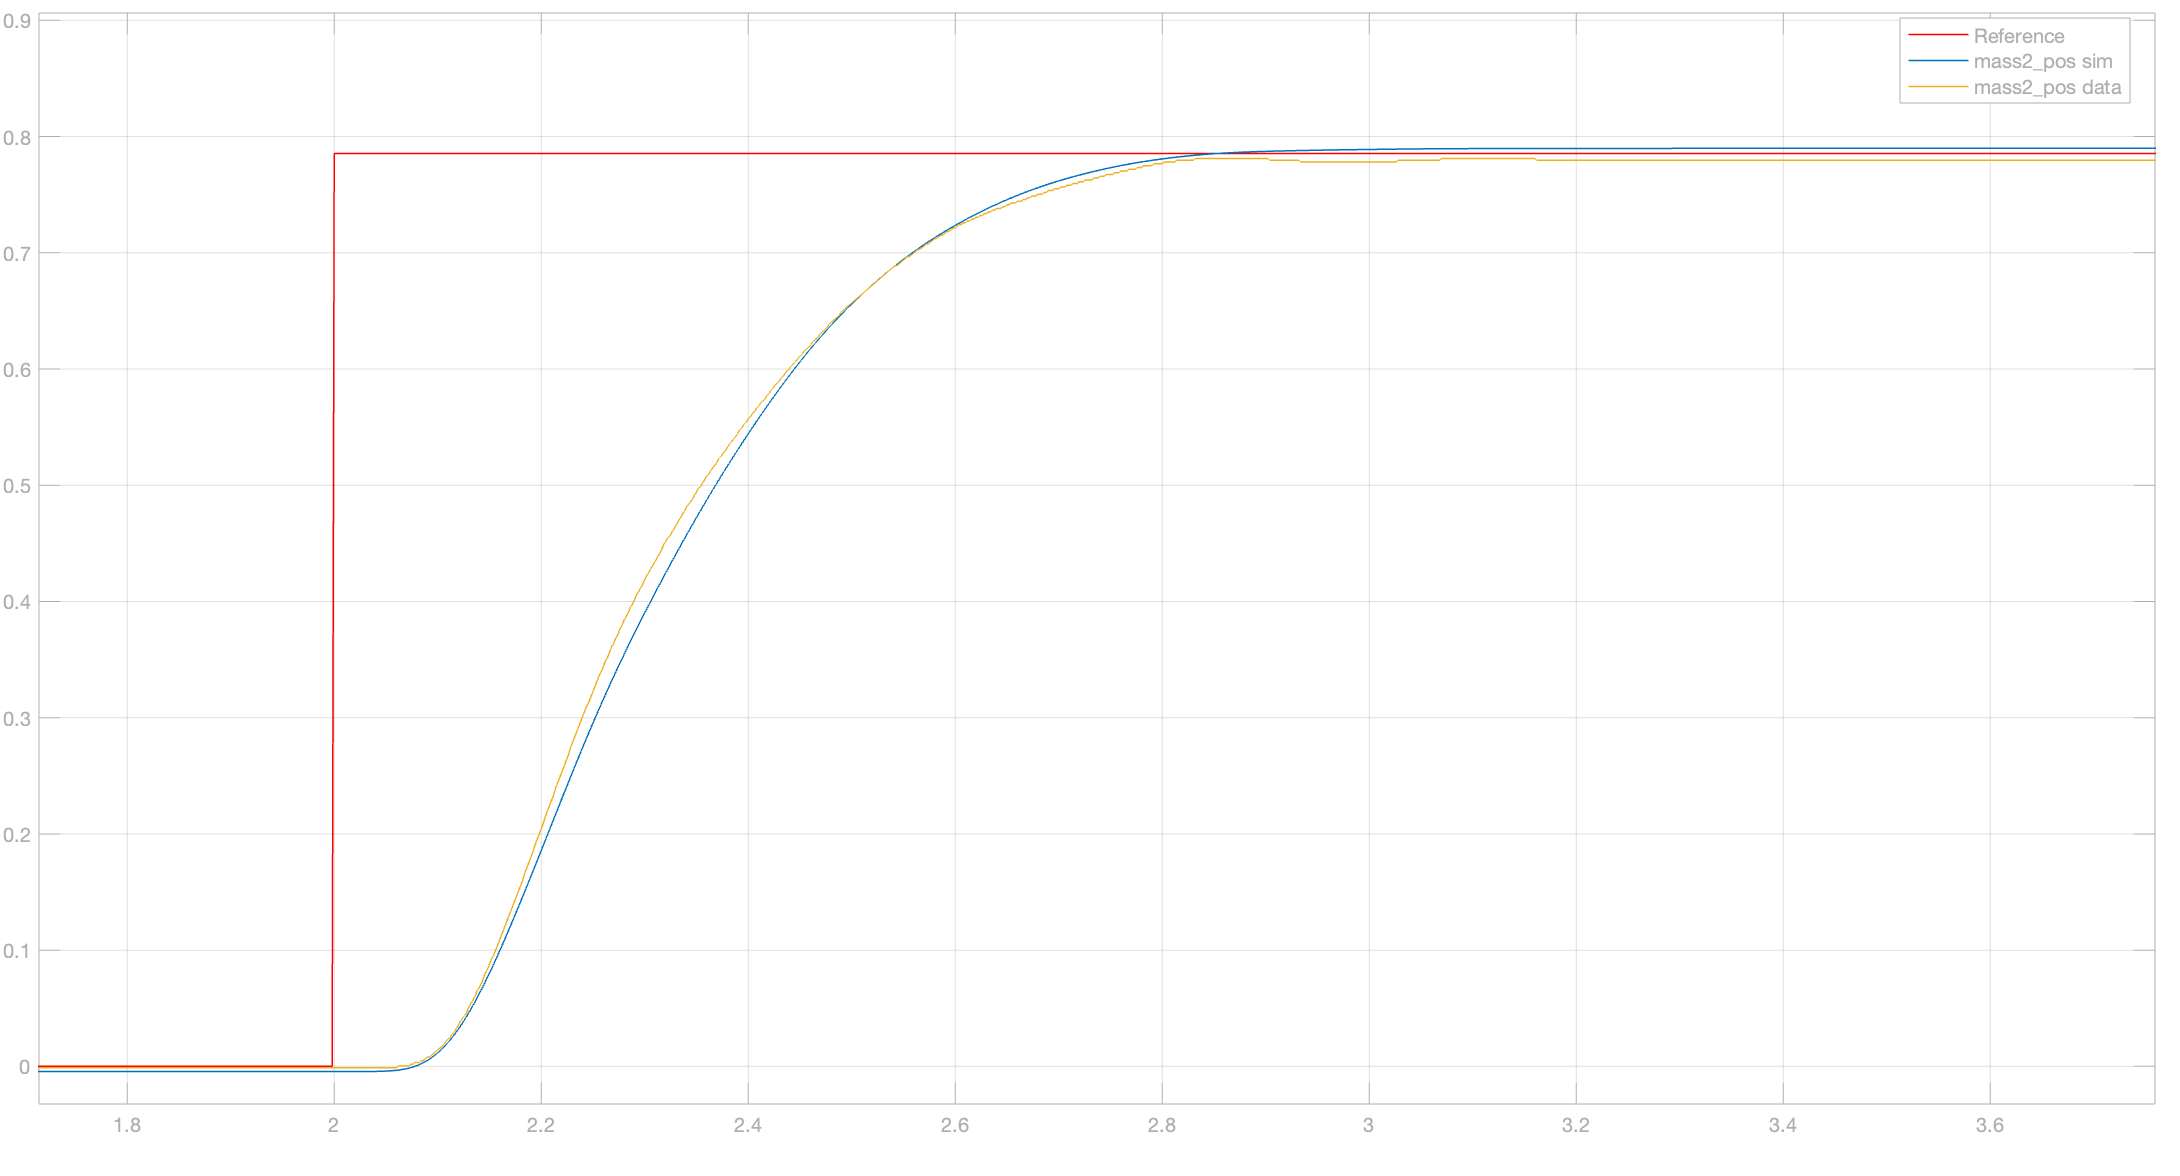
\includegraphics[width=\textwidth]{2dof_LQ_classicKF_focus}
		\subcaption{LQG with all measurements, detail of a step}
		\label{fig:2dof_LQ_classicKF_focus}
	\end{subfigure}
	\caption{LQG with all sensors available, \acrshort{2-dof} case}
	
	\begin{subfigure}{0.45\columnwidth}
		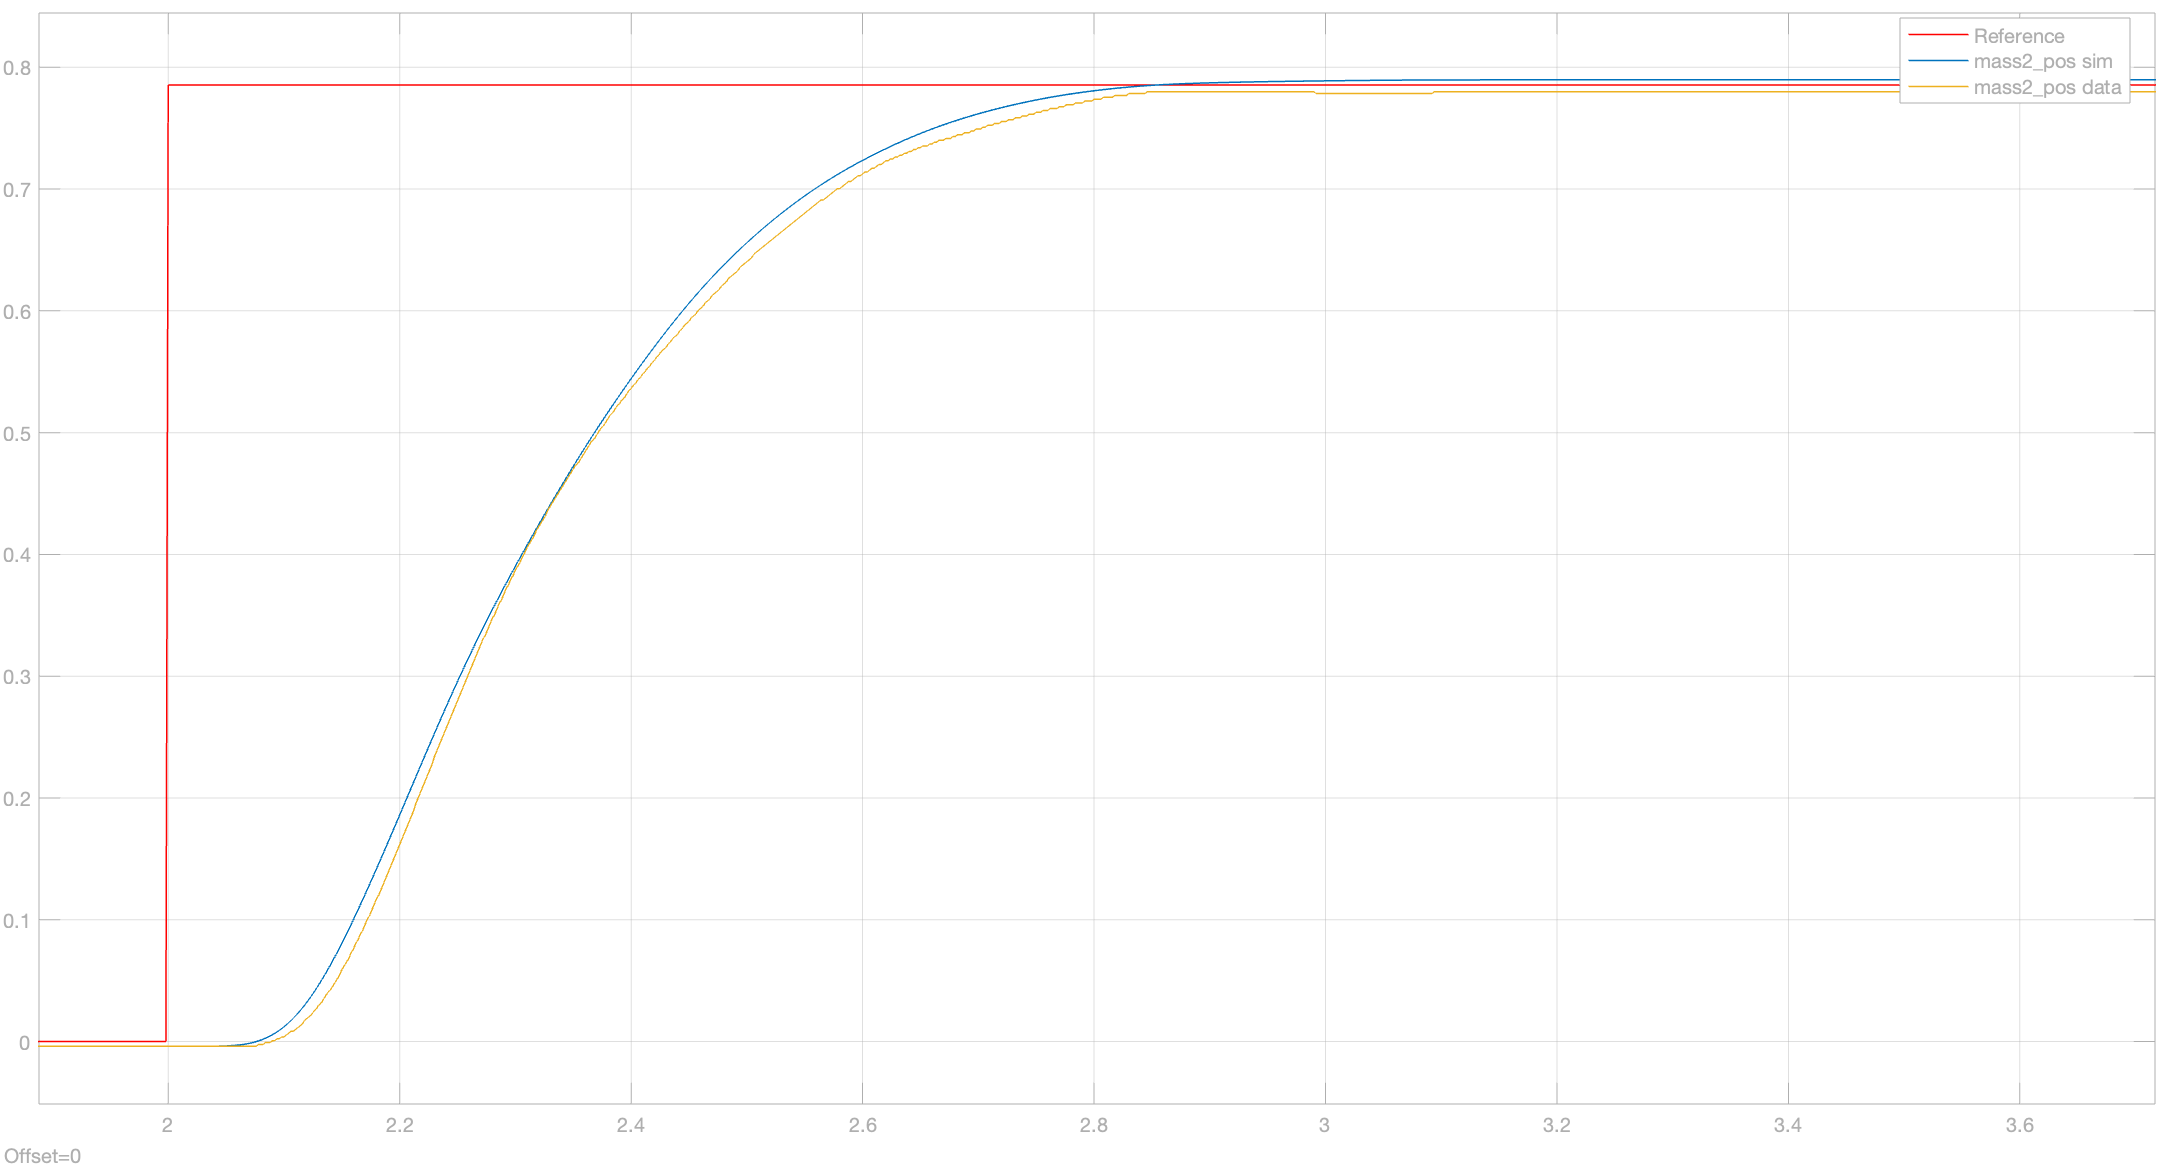
\includegraphics[width=\textwidth]{2dof_LQ_minKF_enc1+enc2}
		\subcaption{LQG with both encoders}
		\label{fig:2dof_LQ_minKF_enc1+enc2}
	\end{subfigure}
	\begin{subfigure}{0.45\columnwidth}
		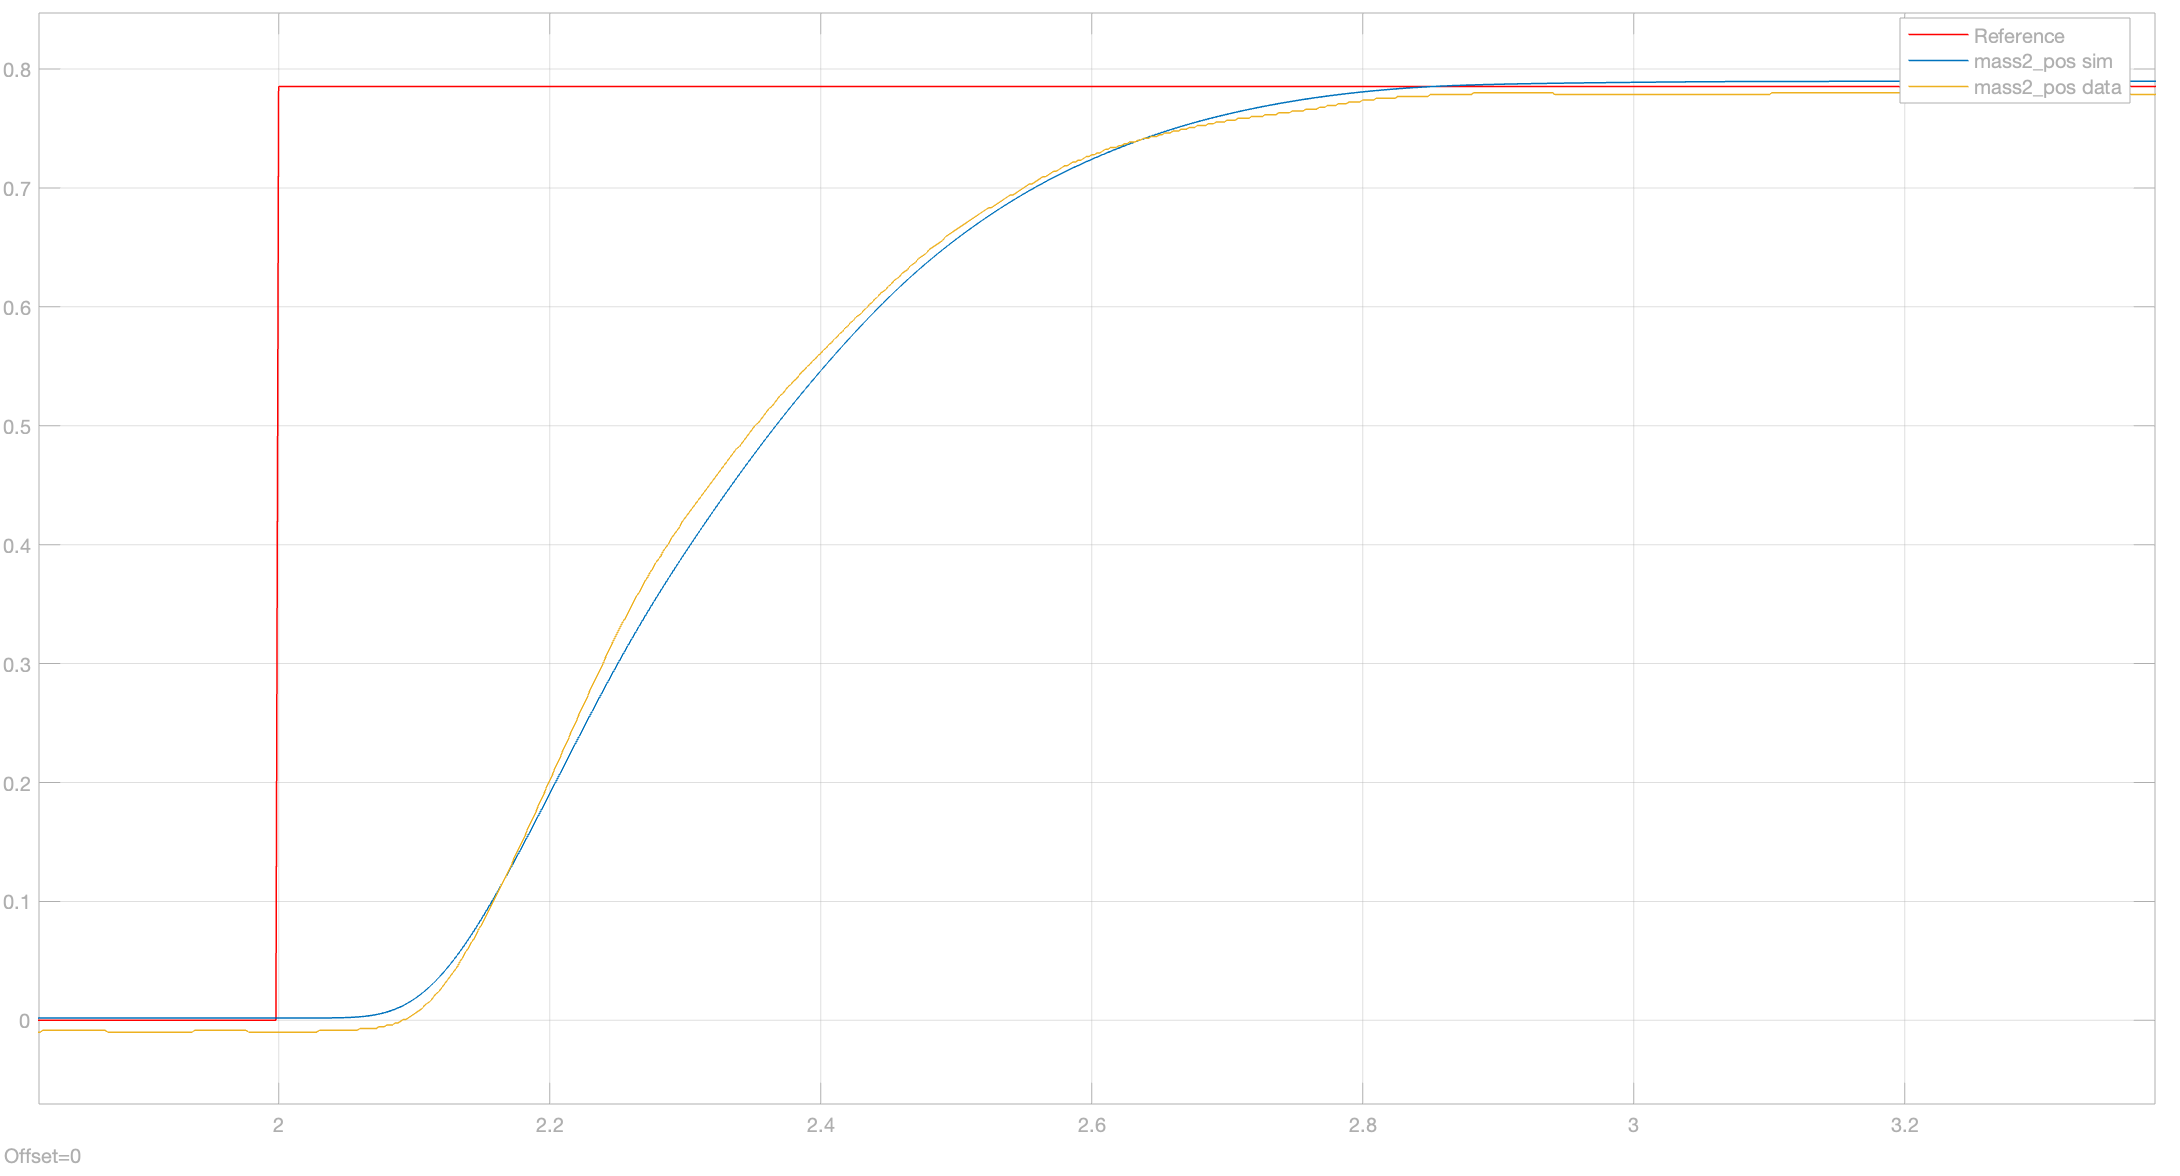
\includegraphics[width=\textwidth]{2dof_LQ_minKF_enc2}
		\subcaption{LQG with second encoder only}
		\label{fig:2dof_LQ_minKF_enc2}
	\end{subfigure}
	\newline
	\begin{subfigure}{0.45\columnwidth}
		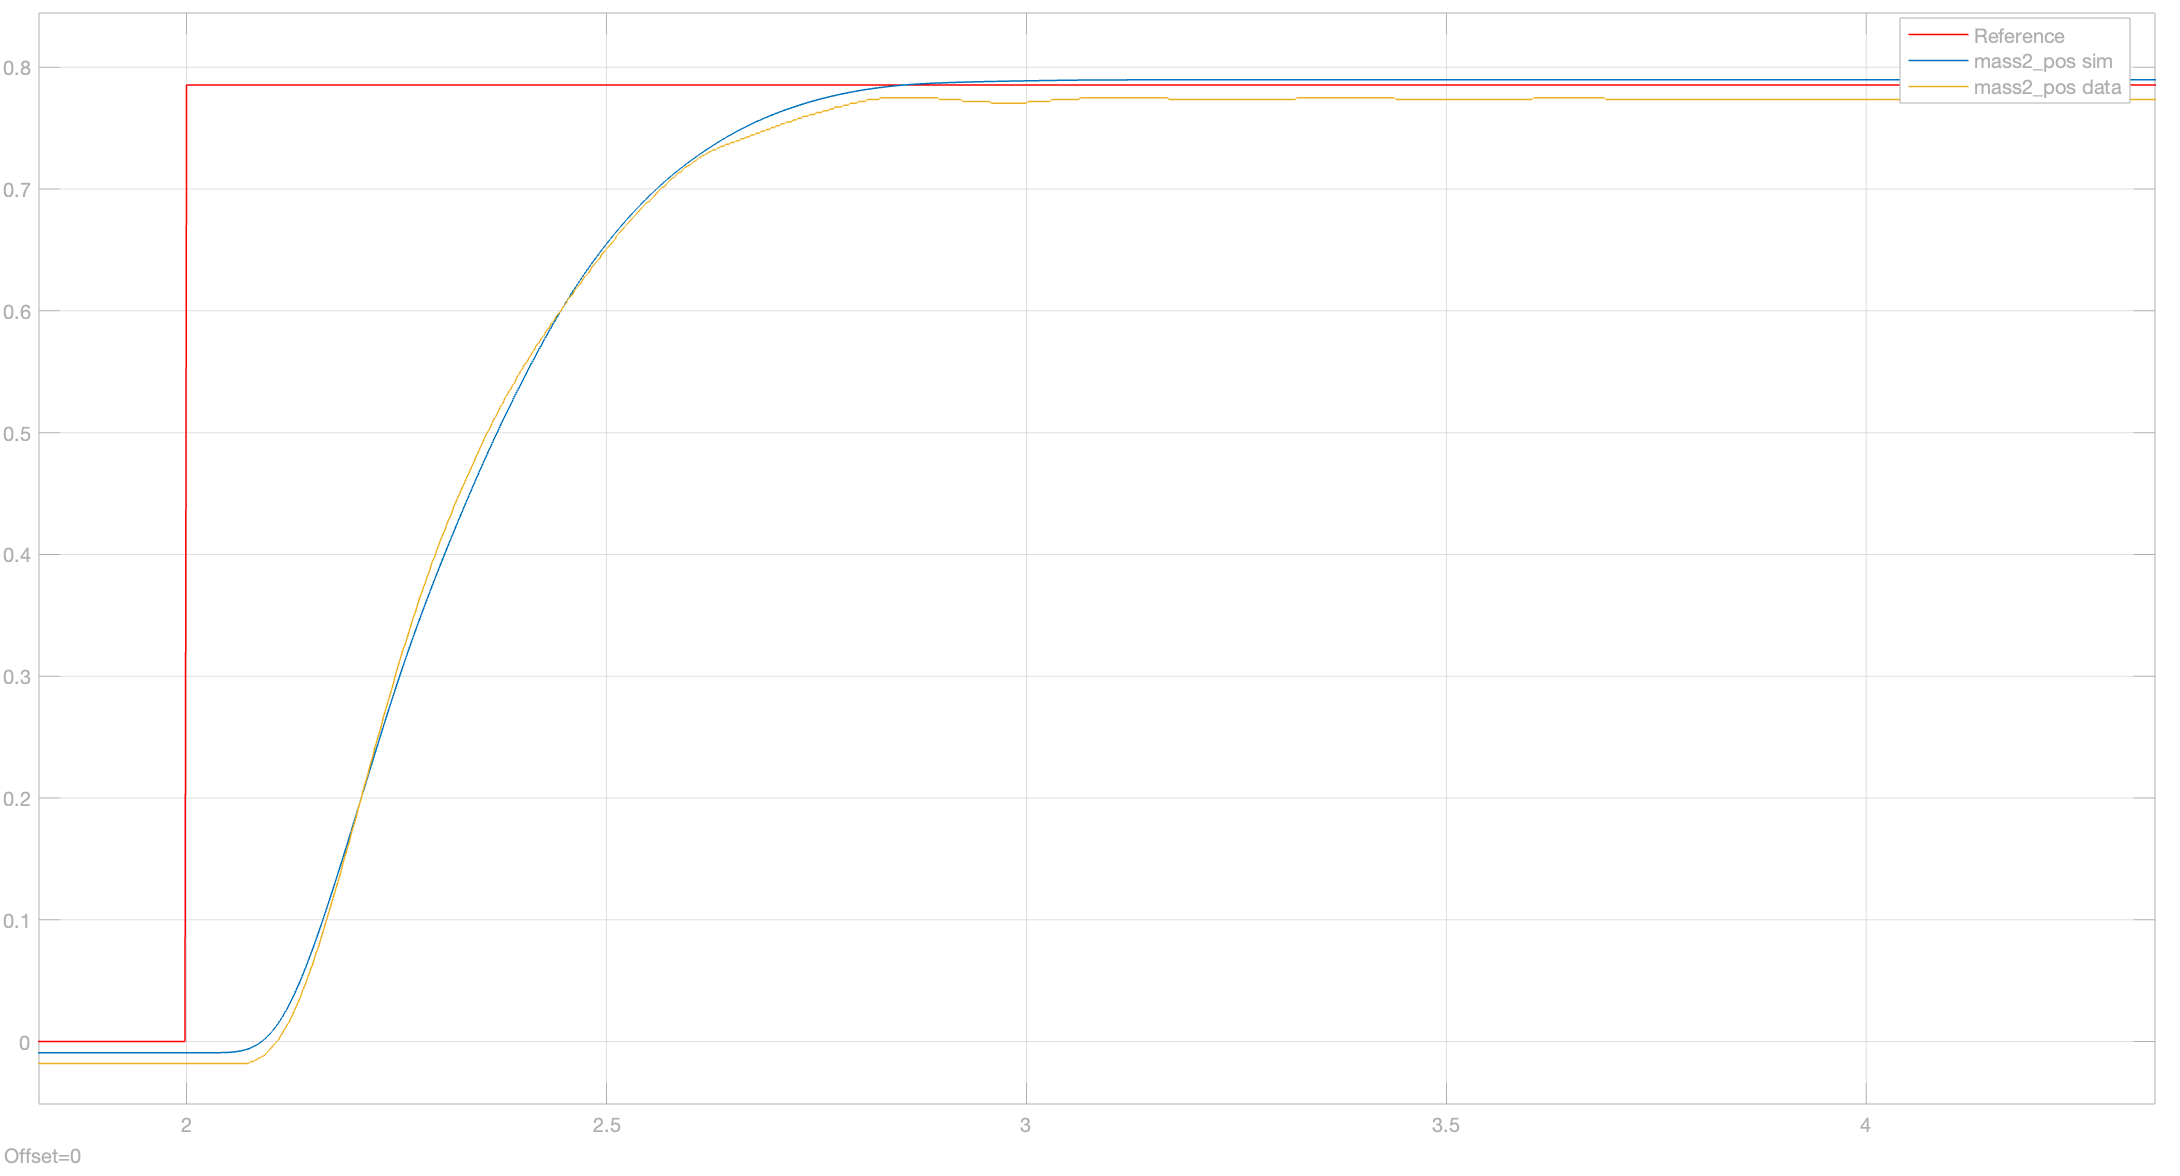
\includegraphics[width=\textwidth]{2dof_LQ_minKF_pot+enc1}
		\subcaption{LQG with potentiometer and first encoder}
		\label{fig:2dof_LQ_minKF_pot+enc1}
	\end{subfigure}
	\begin{subfigure}{0.45\columnwidth}
		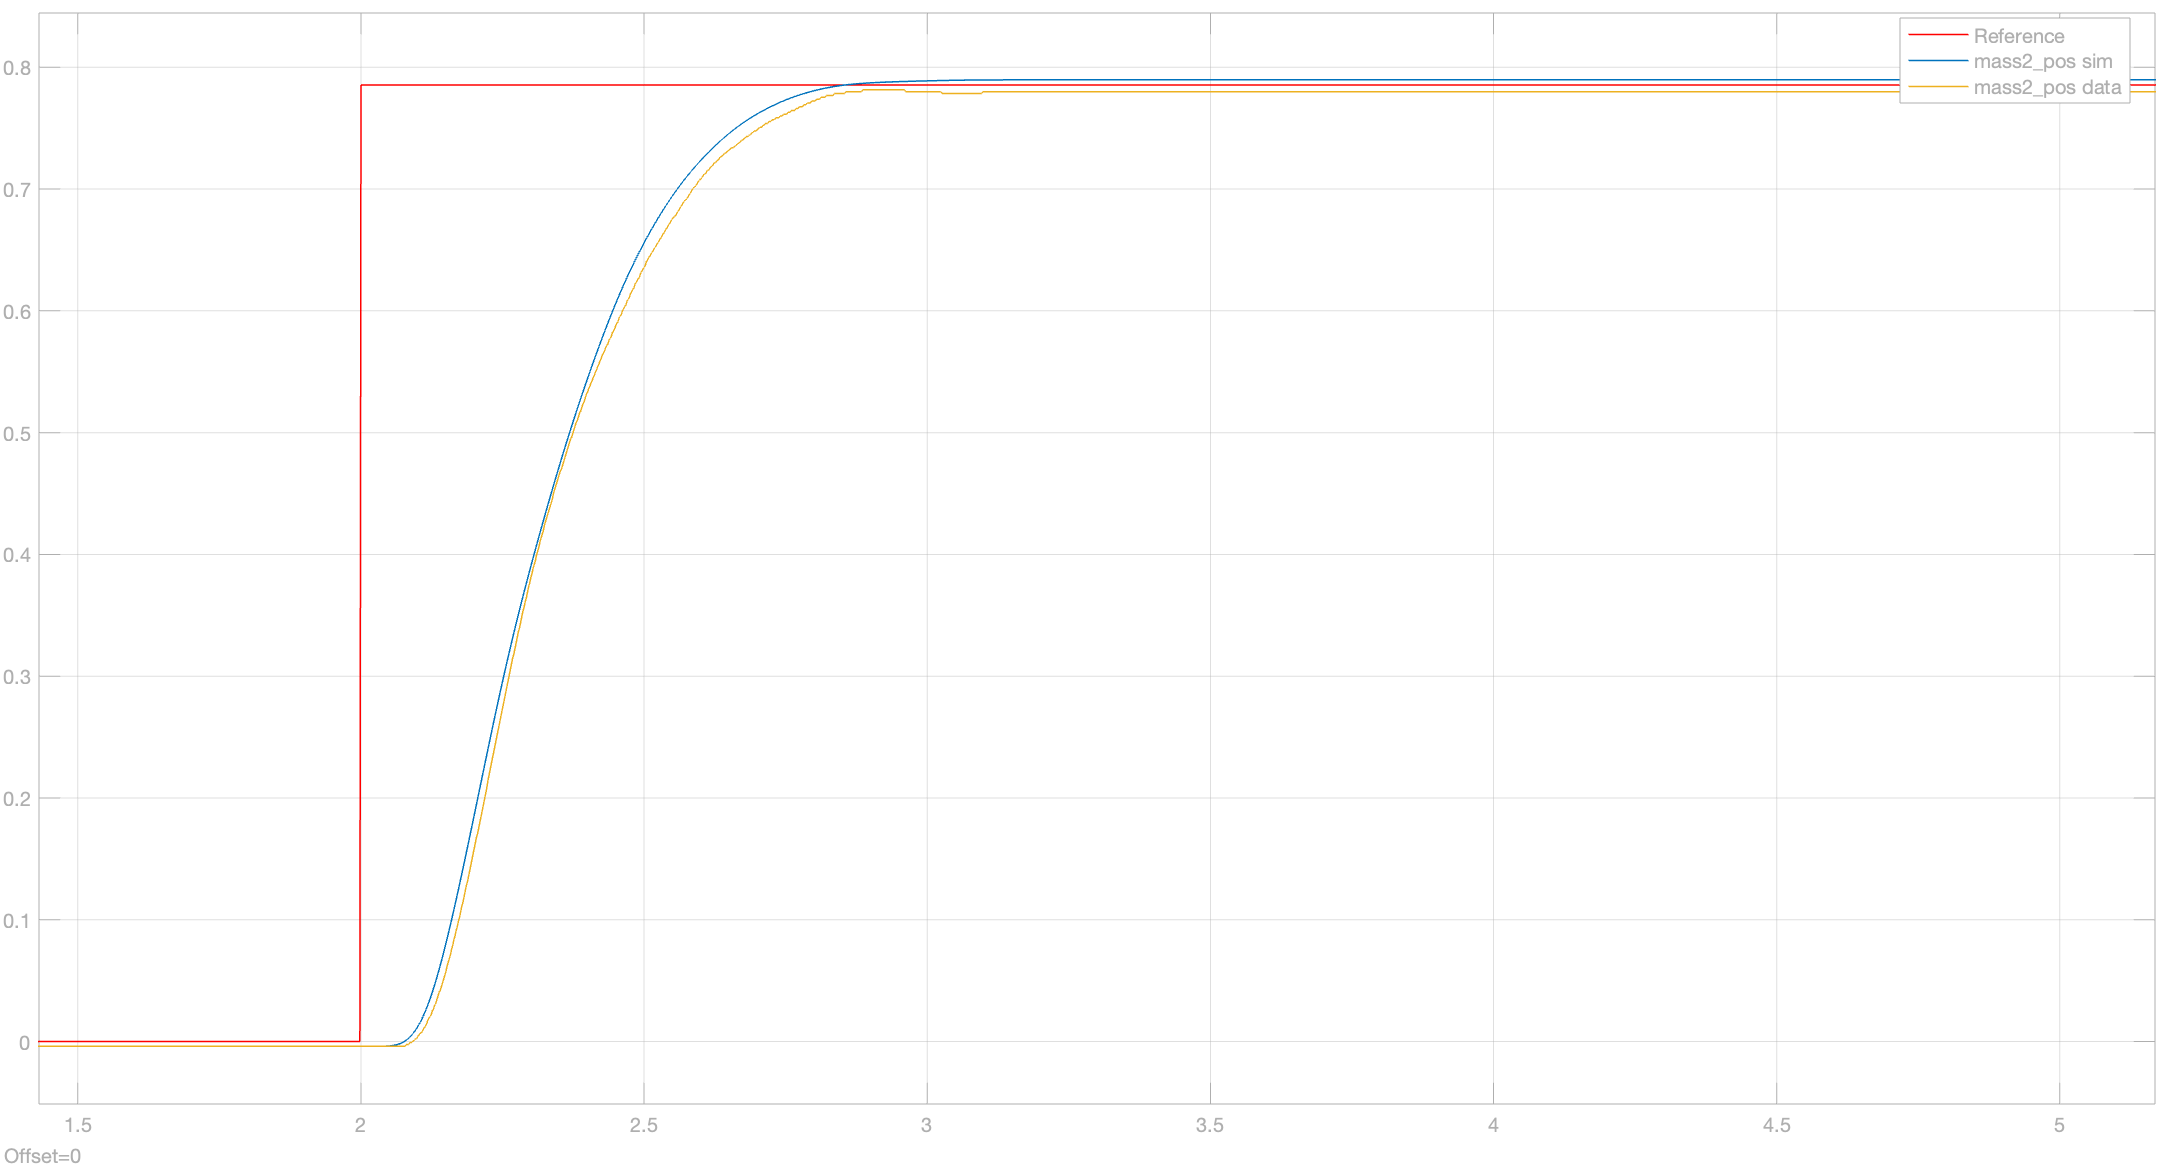
\includegraphics[width=\textwidth]{2dof_LQ_minKF_pot+enc2}
		\subcaption{LQG with potentiometer and second encoder}
		\label{fig:2dof_LQ_minKF_pot+enc2}
	\end{subfigure}
	\caption{LQG with some sensors unavailable, \acrshort{2-dof} case}
	\label{fig:2dof_LQ_minKF}
\end{figure*}
